\begin{surferIntroPage}{World Record Surfaces}{record_chmutovoktic}{Plohe i svjetski rekordi}
Ploha je \emph{nesingularna} ili \emph{glatka} ako ne sadr\v zi vrhove (takve to\v cke zovemo \emph{singulariteti}). Primjeri glatkih ploha su sfera ili torus, \v sto mo\v zete vidjeti na prve 2 slike ispod.
Kada odaberemo neku nasumi\v cnu plohu, u ve\' cini slu\v cajeva \' ce ona biti glatka.
\begin{center}
      \vspace{-0.2cm}
      \begin{tabular}{@{}c@{}c@{}c@{\quad}c@{}c@{}c@{}c@{}}
        \begin{tabular}{@{}c@{}}
          glatke:
        \end{tabular}
        &
        \begin{tabular}{@{}c@{}}
          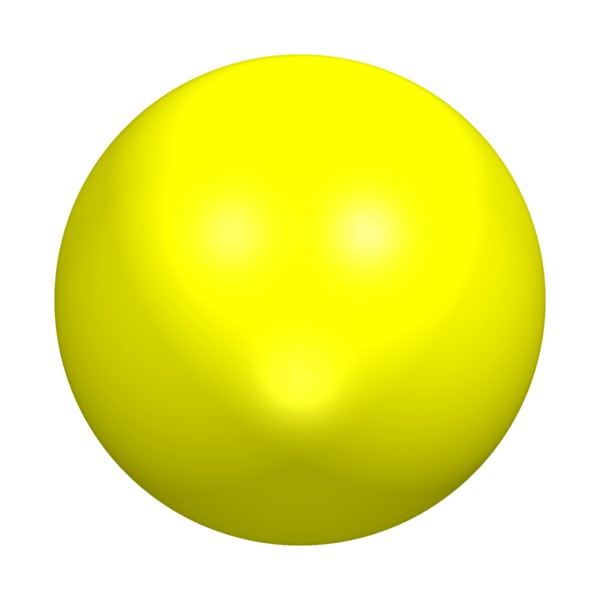
\includegraphics[width=1.1cm]{./../../common/images/kugel}
        \end{tabular}
        &
        \begin{tabular}{@{}c@{}}
          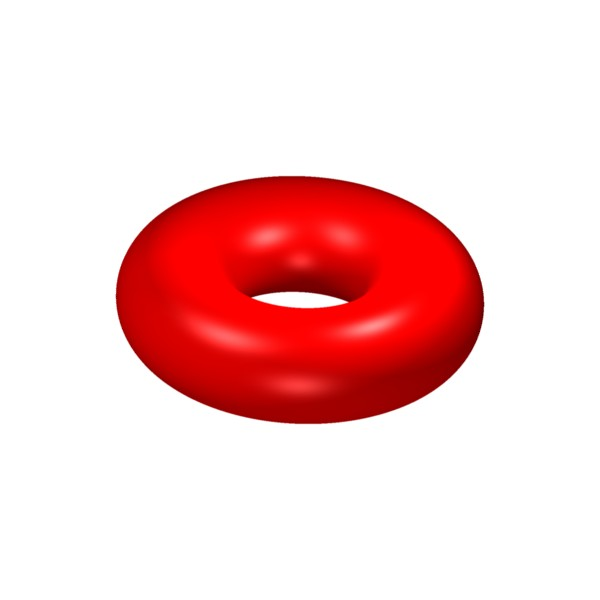
\includegraphics[width=1.1cm]{./../../common/images/torus}
        \end{tabular}
        &
        \begin{tabular}{@{}c@{}}
          puno\\
          singulariteta:
        \end{tabular}
        &
        \begin{tabular}{c@{}@{}}
          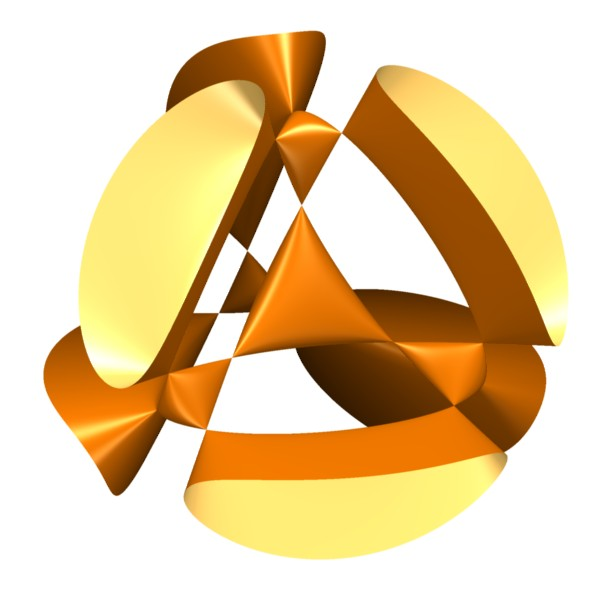
\includegraphics[width=1.1cm]{./../../common/images/kummer}
        \end{tabular}
        &
        \begin{tabular}{c@{}@{}}
          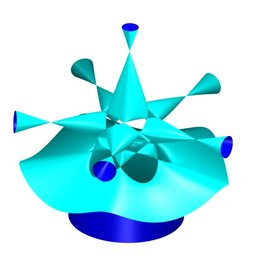
\includegraphics[width=1.1cm]{./../../common/images/togliatti}
        \end{tabular}
        &
        \begin{tabular}{c@{}@{}}
          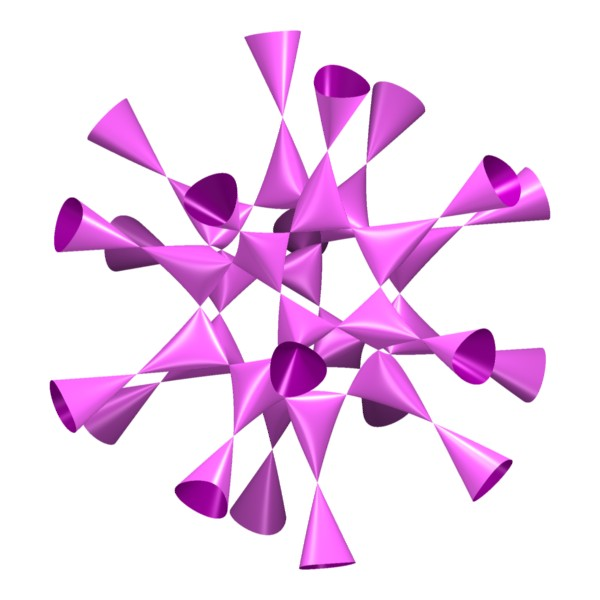
\includegraphics[width=1.1cm]{./../../common/images/barth_sextic}
        \end{tabular}
      \end{tabular}
    \end{center}
    \vspace{-0.2cm}
		Prema tome, posebno zanimljivi slu\v cajevi su oni kada ploha sadr\v zi singularitete jer su to najzanimljivije to\v cke na plohi. Plohe su u aplikaciji SURFER definirane pomo\' cu polinoma. Najve\' ci eksponent polinoma zovemo stupanj polinoma i ozna\v cavamo sa $d$. Matemati\v care \v cesto zanima koliko singulariteta mo\v ze imati ploha odre\dj enog stupnja.
		Taj broj \' cemo ozna\v citi s $\mu(d)$.

Ispostavilo se da je ovaj broj $\mu(d)$ vrlo te\v sko za izra\v cunati.
		Broj $\mu(d)$ je bio poznat jo\v s od $19.$ stolje\' ca za $d=1,2,3,4$, ali za $d=5$ je otkriven tek 1980.\ godine, dok je za $d=6$ otkriven 1996.\ godine.
		Za $d\ge 7$ je broj $\mu(d)$ jo\v s uvijek nepoznat. Poznata nam je samo donja i gornja granica 
		za taj broj.
		
		Prema tome, svako otkri\' ce koje vodi ka preciznijem odre\dj ivanju broja $\mu(d)$ je iznimno va\v zno i predstavlja na neki na\v cin svjetski rekord. Potrebno je jako puno vremena za rije\v siti u potpunosti ovaj problem za proizvoljni $d$.\\ Neki dosad poznati rezultati su:
		
		\begin{center}
      \begin{tabular}{r|cccccccc|c}
        $d$ & $1$ & $2$ & $3$ & $4$ & $5$ & $6$ & $7$ & $8$ & $d$\\
        \hline
        \hline
        \rule{0pt}{1.2em}$\mu(d)\ge$ & $0$ & $1$ & $4$ & $16$ & $31$ & $65$ &
        $99$ & $168$ & 
        $\approx \frac{5}{12}d^3$\\[0.3em]
        \hline
        \rule{0pt}{1.2em}$\mu(d)\le$ & $0$ & $1$ & $4$ & $16$ & $31$ & $65$ &
        $104$ & $174$ & $\approx \frac{4}{9}d^3$
      \end{tabular}
    \end{center}
\end{surferIntroPage}
